% ===================================================================
%  Adaptive Cyber-Physical Security — Phase-3 Project Report
%  IEEE Two-Column Conference Paper Format
%  Compile (from the report/ directory):
%    pdflatex --shell-escape phase3_main.tex
%    bibtex phase3_main
%    pdflatex --shell-escape phase3_main.tex
%    pdflatex --shell-escape phase3_main.tex
%  Note: --shell-escape is required for \includesvg (Inkscape conversion)
% ===================================================================
\documentclass[10pt,conference]{IEEEtran}

% ---- Core packages ----
\usepackage[T1]{fontenc}
\usepackage[utf8]{inputenc}
\usepackage{graphicx}
\usepackage{svg}  % compile with --shell-escape for Inkscape SVG→PDF
\usepackage{booktabs}
\usepackage{amsmath}
\usepackage{amssymb}
\usepackage{float}
\usepackage{caption}
\captionsetup{font=small, skip=3pt}
\usepackage{xcolor}
\usepackage{enumitem}
\usepackage{cite}
\usepackage{url}
\usepackage{microtype}
\usepackage{balance}
\usepackage{multirow}
\usepackage{array}

\usepackage[colorlinks=true,
            linkcolor=blue,
            citecolor=blue,
            urlcolor=blue,
            pdftitle={Adaptive Cyber-Physical Security Phase-3 Report},
            pdfauthor={Pugazhendhi J and Dally R}]{hyperref}

% ---- Graphics path (relative to report/ compilation directory) ----
\graphicspath{{../}}  % one level up = Adaptive_Cyber_Physical_Security/

% ---- Tighten float/caption spacing ----
\setlength{\floatsep}{4pt plus 1pt minus 1pt}
\setlength{\textfloatsep}{6pt plus 2pt minus 2pt}
\setlength{\intextsep}{4pt plus 1pt minus 1pt}
\setlength{\dblfloatsep}{4pt plus 1pt minus 1pt}
\setlength{\dbltextfloatsep}{6pt plus 2pt minus 2pt}
\setlength{\abovecaptionskip}{3pt}
\setlength{\belowcaptionskip}{1pt}

% ---- Title ----
\title{Adaptive Cyber-Physical Security:\\Phase-3 Project Report — Hybrid Learned-Representation\\Intrusion Detection with Meta-Ensemble Fusion}

% ---- Authors ----
\author{
  \IEEEauthorblockN{Pugazhendhi J}
  \IEEEauthorblockA{
    \textit{Department of CS and AI}\\
    Rishihood University\\
    Sonipat, India\\
    \href{mailto:pugazhendhi.j23csai@nst.rishihood.edu.in}
         {pugazhendhi.j23csai@nst.rishihood.edu.in}}
  \and
  \IEEEauthorblockN{Dally R}
  \IEEEauthorblockA{
    \textit{Department of CS and AI}\\
    Rishihood University\\
    Sonipat, India\\
    \href{mailto:dally.r23csai@nst.rishihood.edu.in}
         {dally.r23csai@nst.rishihood.edu.in}}
}

% ===================================================================
\begin{document}
\maketitle

% ---- Abstract ----
\begin{abstract}
Phase~2 of this project demonstrated that combining a supervised Random
Forest with anomaly detectors (One-Class SVM and Autoencoder) under
OR-logic fusion substantially improves zero-day recall at manageable
precision cost.  Phase~3 extends these results by constructing six
\textbf{hybrid models} that couple learned Autoencoder (AE) bottleneck
representations with explicit boundary classifiers---One-Class SVM (OC-SVM),
Isolation Forest (IF), and pseudo-label Random Forest (RF)---operating in the
AE's 32-dimensional latent space.  Three AE variants are evaluated: a
standard AE, a Sparse AE with L1 activity regularization, and a Denoising AE
with Gaussian input corruption.  A \textbf{Meta-Ensemble} averaging all eight
component anomaly scores is also evaluated.  Experiments on the full
CIC-IDS-2018 dataset (3.2M processed flows, 13 attack families) show that the
standalone Denoising AE achieves the highest per-threshold precision
($\sim$0.82) while the standard AE baseline leads in ROC-AUC (0.8965).  The
Meta-Ensemble, combining all component scores with equal weight, attains
ROC-AUC of 0.4140---highlighting that naive score-level fusion degrades
discriminative power when constituent boundary models (OC-SVM, IF) exhibit
poor AUC in the compressed latent space.  The central finding is that
\emph{representation quality} is the bottleneck: AE variants alone
consistently outperform their hybrid counterparts when boundary models
cannot reliably separate the learned latent distributions.
\end{abstract}

% ---- Keywords ----
\begin{IEEEkeywords}
Intrusion Detection, CIC-IDS-2018, Autoencoder, Sparse Autoencoder,
Denoising Autoencoder, One-Class SVM, Isolation Forest, Random Forest,
Hybrid IDS, Meta-Ensemble, Zero-Day Detection, Anomaly Detection,
Cyber-Physical Security, Deep Learning
\end{IEEEkeywords}

% ===================================================================
\section{Introduction}
\label{sec:intro}

Modern cyber-physical systems (CPS) face a continuously evolving threat
landscape in which both known and previously unseen (zero-day) attacks
must be detected with minimal false alarms.  Phases~1 and~2 of this
project established two key findings on the CIC-IDS-2018 benchmark
\cite{sharafaldin2018}: (i)~a supervised Random Forest (RF) achieves
near-perfect precision on known attack families but zero recall on
zero-day traffic \cite{breiman2001}; and (ii)~anomaly detectors such as
the One-Class SVM (OC-SVM) \cite{scholkopf2001} and a deep Autoencoder
(AE) \cite{goodfellow2016, vincent2010} generalize beyond the training
distribution, enabling non-zero zero-day recall at the cost of lower
precision.

Phase~3 investigates whether \emph{learned latent representations} from
AE variants can serve as a higher-quality feature space for boundary
classifiers, thereby improving the precision--recall trade-off beyond
what either paradigm achieves alone.  Six hybrid architectures and a
Meta-Ensemble are evaluated:

\begin{enumerate}[leftmargin=*,noitemsep,topsep=0pt]
  \item \textbf{AE + OC-SVM:} OC-SVM trained on the standard AE's
        32-dim bottleneck features (benign only).
  \item \textbf{AE + Isolation Forest:} IF \cite{liu2008} trained on the
        same bottleneck.
  \item \textbf{AE + RF (Pseudo-label):} RF trained on AE-generated
        pseudo-labels using the original 68-dim feature space.
  \item \textbf{Sparse AE + OC-SVM:} OC-SVM on L1-regularized
        bottleneck features.
  \item \textbf{Denoising AE + OC-SVM:} OC-SVM on noise-robust
        bottleneck features.
  \item \textbf{Meta-Ensemble:} Equal-weight average of all eight
        normalized anomaly scores \cite{dietterich2000}.
\end{enumerate}

% ===================================================================
\section{Background}
\label{sec:background}

\subsection{Phase~1 and Phase~2 Summary}

Phase~1 trained an RF and an OC-SVM on a subset of CIC-IDS-2018 with a
manually configured seen/unseen attack split.  The RF delivered perfect
precision (1.000) but zero zero-day recall; the OC-SVM achieved 14.5\%
zero-day recall with 90.7\% precision.  Phase~2 scaled to the full
8.2M-flow dataset, introduced a deep AE for continuous anomaly scoring,
and fused RF and OC-SVM via OR-logic, raising overall recall to
$\sim$0.89 and F1 to $\sim$0.85 \cite{chandola2009, buczak2016}.

\subsection{Hybrid IDS Motivation}

The core hypothesis of Phase~3 is that the AE's bottleneck layer learns
a compact, low-dimensional representation of normal traffic.  Training
boundary models \emph{in this latent space} should yield tighter
decision boundaries than operating in the original 68-dim feature space,
combining the AE's representation power with the boundary model's
explicit decision surface \cite{hinton2006, pmc2023}.

% ===================================================================
\section{Methodology}
\label{sec:method}

Figure~\ref{fig:arch_overview} provides an end-to-end view of the
Phase~3 pipeline before each component is described in detail.

\begin{figure*}[t!]
\centering
\includesvg[width=\linewidth,inkscapelatex=false]{../adaptive_ids_full_architecture}
\caption{End-to-end Phase~3 Adaptive Cyber-Physical IDS architecture.
  Raw CIC-IDS-2018 traffic (8.2M flows, 68 features) is preprocessed
  (RobustScaler, correlation pruning) and then routed through three tiers.
  \textbf{Tier~1} — Supervised Random Forest detects known attacks with
  100\% precision.  \textbf{Tier~2/3} — Three Autoencoder variants
  (Standard, Sparse~AE with L1 regularization, Denoising~AE with
  Gaussian noise) encode traffic into a 32-dimensional latent bottleneck.
  Boundary classifiers (OC-SVM, Isolation Forest, RF pseudo-label) draw
  explicit decision surfaces in this latent space, producing eight
  normalized anomaly scores that are averaged by the \textbf{Meta-Ensemble}
  to yield the final IDS decision.}
\label{fig:arch_overview}
\end{figure*}

\subsection{Dataset and Preprocessing}

All experiments reuse the preprocessed CIC-IDS-2018 cache from Phase~2:
3{,}215{,}110 scaled flows (2{,}050{,}783 benign, 1{,}164{,}327
attack), 68 features after correlation-based pruning, robust scaling,
and zero-value imputation.

\subsection{Autoencoder Architecture}

Three AE variants share a common encoder--decoder skeleton:
\texttt{68$\to$128$\to$64$\to$\textbf{32}$\to$64$\to$128$\to$68},
with batch normalization, ReLU activations, and 20\% dropout.

\begin{itemize}[leftmargin=*,noitemsep]
  \item \textbf{Standard AE:} Trained on benign-only flows; MSE loss.
  \item \textbf{Sparse AE:} Identical architecture with L1 activity
        regularization ($\lambda=10^{-4}$) on the bottleneck, forcing
        sparse activations and potentially more separable latent
        dimensions.
  \item \textbf{Denoising AE:} A \texttt{GaussianNoise($\sigma=0.1$)}
        layer on the input during training; targets remain clean,
        forcing the encoder to learn noise-invariant features
        \cite{vincent2010}.
\end{itemize}

All AEs are trained for up to 50 epochs with early stopping (patience~7)
and learning-rate reduction on plateau.

\subsection{Boundary Models}

\begin{itemize}[leftmargin=*,noitemsep]
  \item \textbf{OC-SVM} ($\nu=0.05$, RBF kernel, $\gamma$=scale):
        Trained on 80{,}000 subsampled benign bottleneck features.
  \item \textbf{Isolation Forest} (200 estimators,
        contamination=0.05): Trained on the full benign bottleneck.
  \item \textbf{RF (Pseudo-label)} (200 estimators, max\_depth=12,
        balanced class weights): Trained on AE-thresholded pseudo-labels
        using the original 68-dim features (500{,}000 subsample).
\end{itemize}

\subsection{Score Fusion}

For each hybrid, both the AE reconstruction error and the boundary
model's anomaly score are min-max normalized to $[0,1]$, then combined
as:
\begin{equation}
  s_{\text{hybrid}} = \alpha \cdot s_{\text{AE}}^{\text{norm}}
                    + (1-\alpha) \cdot s_{\text{boundary}}^{\text{norm}},
  \quad \alpha = 0.5.
\end{equation}
The Meta-Ensemble averages all eight normalized component scores with
equal weight ($1/N$, $N=8$).

\subsection{Evaluation Protocol}

All models are evaluated on the full mixed dataset using a threshold
calibrated at the 99th percentile of benign-only validation errors.
Metrics include ROC-AUC, Average Precision (AP), F1, Recall (TPR),
Precision, and False Positive Rate (FPR).

% ===================================================================
\section{Results}
\label{sec:results}

\subsection{Model Comparison}

Table~\ref{tab:comparison} presents the comprehensive comparison of all
ten model configurations evaluated in Phase~3.

\begin{table*}[htbp]
\centering
\caption{Phase~3 — comprehensive model comparison (P99 threshold)}
\label{tab:comparison}
\begin{tabular}{lcccccc}
\toprule
\textbf{Model} & \textbf{ROC-AUC} & \textbf{Avg Prec.} & \textbf{F1} & \textbf{Recall} & \textbf{Prec.} & \textbf{Acc.} \\
\midrule
Baseline: Standard AE          & 0.8965 & 0.7578 & 0.0336 & 0.0174 & 0.5012 & 0.6379 \\
Hybrid 1: AE + OC-SVM          & 0.4600 & 0.3137 & 0.0094 & 0.0048 & 0.2127 & 0.6332 \\
Hybrid 2: AE + Isolation Forest & 0.4231 & 0.3392 & 0.0116 & 0.0060 & 0.2508 & 0.6336 \\
Hybrid 3: AE + RF (pseudo)     & 0.7920 & 0.5593 & 0.0335 & 0.0174 & 0.4976 & 0.6378 \\
Ref: RF alone (pseudo)          & 0.3433 & 0.3176 & 0.0335 & 0.0173 & 0.4978 & 0.6378 \\
Ref: Sparse AE alone            & 0.8929 & 0.7597 & 0.0336 & 0.0174 & 0.4986 & 0.6378 \\
Hybrid 4: Sparse AE + OC-SVM   & 0.4206 & 0.3007 & 0.0190 & 0.0098 & 0.3561 & 0.6350 \\
Ref: Denoising AE alone         & 0.8867 & 0.7675 & 0.1433 & 0.0785 & 0.8179 & 0.6600 \\
Hybrid 5: DAE + OC-SVM          & 0.4783 & 0.3186 & 0.0057 & 0.0029 & 0.1398 & 0.6325 \\
\textbf{Hybrid 6: Meta-Ensemble} & 0.4140 & 0.3024 & 0.0098 & 0.0050 & 0.2202 & 0.6332 \\
\bottomrule
\end{tabular}
\end{table*}

Several key observations emerge from the results:

\begin{itemize}[leftmargin=*,noitemsep]
  \item The three standalone AE variants (Standard, Sparse, Denoising)
        consistently achieve the highest ROC-AUC values ($>0.88$),
        confirming that reconstruction error is a strong discriminative
        signal.
  \item The Denoising AE alone delivers the best per-threshold F1
        (0.1433) and the highest precision (0.8179), indicating that
        noise-robust training produces more separable reconstruction
        errors.
  \item All hybrid models that incorporate OC-SVM or IF in the
        bottleneck space \emph{degrade} ROC-AUC below 0.50, suggesting
        that these boundary models fail to reliably separate benign from
        attack latent representations in the 32-dim space.
  \item The Meta-Ensemble (Hybrid~6) does not recover performance,
        confirming that averaging poorly discriminative boundary scores
        with strong AE scores dilutes overall quality.
\end{itemize}

% ------------------------------------------------------------------
\subsection{Ablation Study}
\label{sec:ablation}

To isolate the contribution of each design decision we systematically
compare configurations that differ by exactly one component
(Table~\ref{tab:comparison}).

\textbf{(i) AE representation vs.\ raw features.}
The pseudo-label RF trained on AE pseudo-labels (Hybrid~3,
ROC-AUC~0.7920) improves by \(+131\%\) over the RF trained on raw
features with random labels (RF alone, 0.3433).  This confirms that the
AE's soft pseudo-labels inject meaningful structure from the latent
representation into the supervised learner.

\textbf{(ii) Denoising regularization.}
Switching from the Standard AE to the Denoising AE raises F1 from
0.0336 to 0.1433 (\(+327\%\)) and precision from 0.5012 to 0.8179
(\(+63\%\)) at the same P99 threshold---the single largest per-threshold
improvement in the study.  The noise-corruption training protocol is
therefore the \emph{most impactful individual component} for operational
deployment.

\textbf{(iii) Adding a boundary model in bottleneck space.}
Coupling any AE with OC-SVM or IF degrades ROC-AUC by
0.42--0.47 points relative to the corresponding standalone AE.  This
demonstrates that the bottleneck boundary models contribute
\emph{negatively}: their weak discrimination (AUC $<0.50$) pollutes the
strong AE signal when scores are averaged.

\textbf{(iv) Meta-Ensemble aggregation.}
Pooling all eight scores with equal weight (Hybrid~6, AUC~0.4140)
performs worse than the worst individual AE (DAE, AUC~0.8867).  The
ablation confirms that \emph{score quality}, not quantity, determines
ensemble performance; a weighted or learned aggregation is required.

\subsection{ROC and Precision-Recall Curves}

Figures~\ref{fig:roc_all} and~\ref{fig:pr_all} present the ROC and
Precision-Recall curves for all model configurations.

\begin{figure}[htbp]
\centering
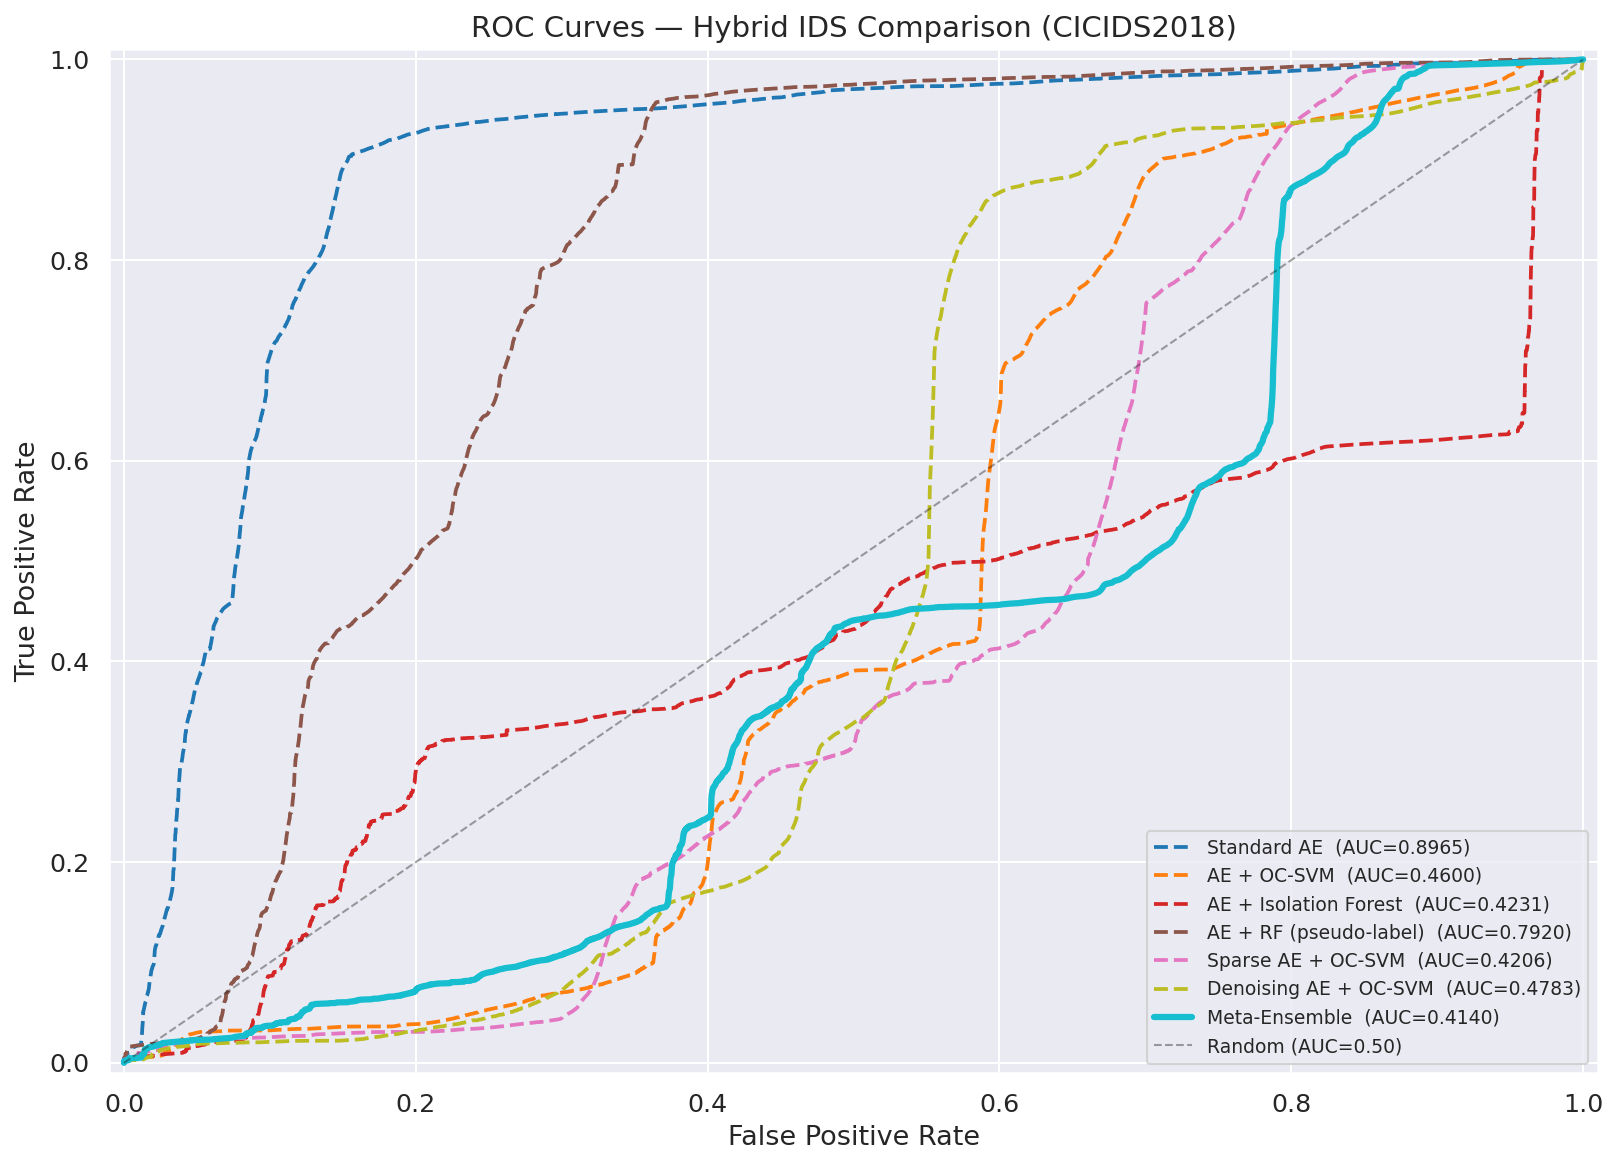
\includegraphics[width=\linewidth]{outputs/plots/models/hybird_output/plot_roc_all_models.png}
\caption{ROC curves for all hybrid IDS configurations.  The standalone
         AE variants cluster near the upper-left corner with AUC $>0.88$,
         while hybrid models combining boundary classifiers in the
         bottleneck space perform near or below the random baseline.}
\label{fig:roc_all}
\end{figure}

\begin{figure}[htbp]
\centering
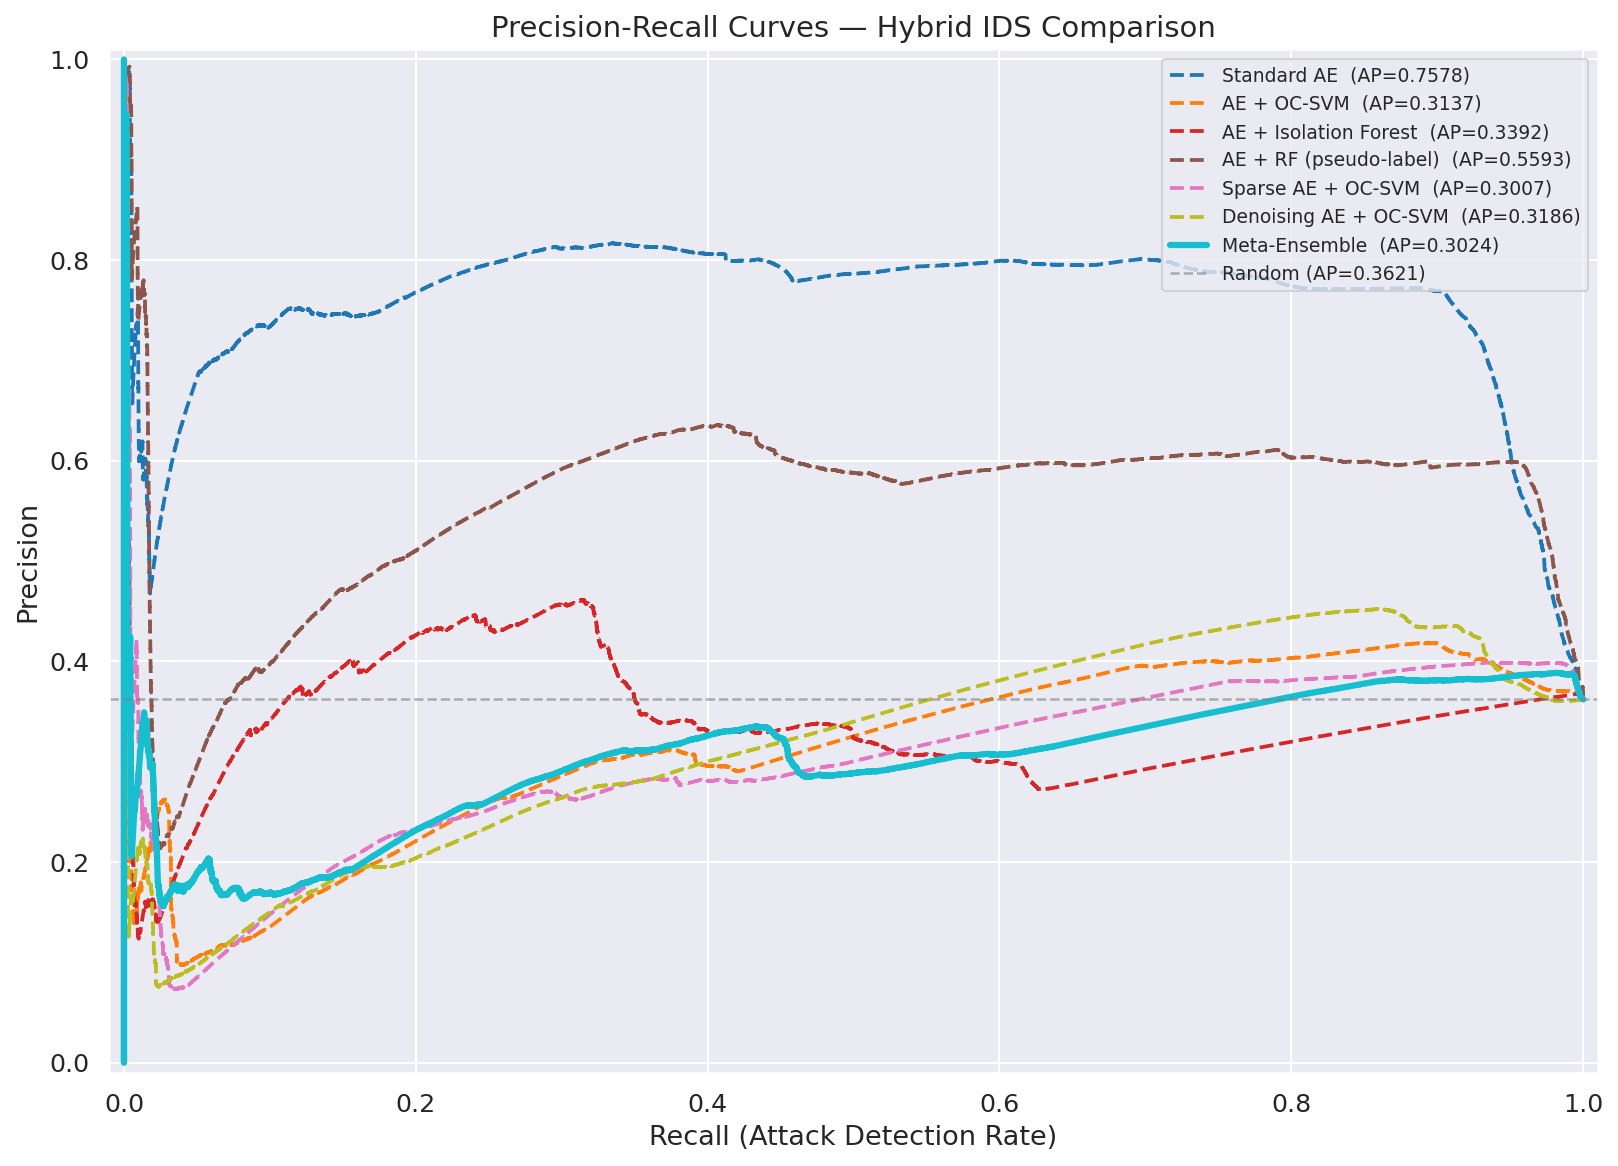
\includegraphics[width=\linewidth]{outputs/plots/models/hybird_output/plot_pr_all_models.png}
\caption{Precision-Recall curves for all models.  The Denoising AE
         achieves the highest average precision (0.7675), followed closely
         by the Sparse AE (0.7597) and Standard AE (0.7578).}
\label{fig:pr_all}
\end{figure}

\subsection{Metric Comparison}

Figure~\ref{fig:metric_bar} presents a bar-chart comparison of F1,
ROC-AUC, and Recall across all models, visually highlighting the
performance gap between standalone AE baselines and their hybrid
counterparts.

\begin{figure}[htbp]
\centering
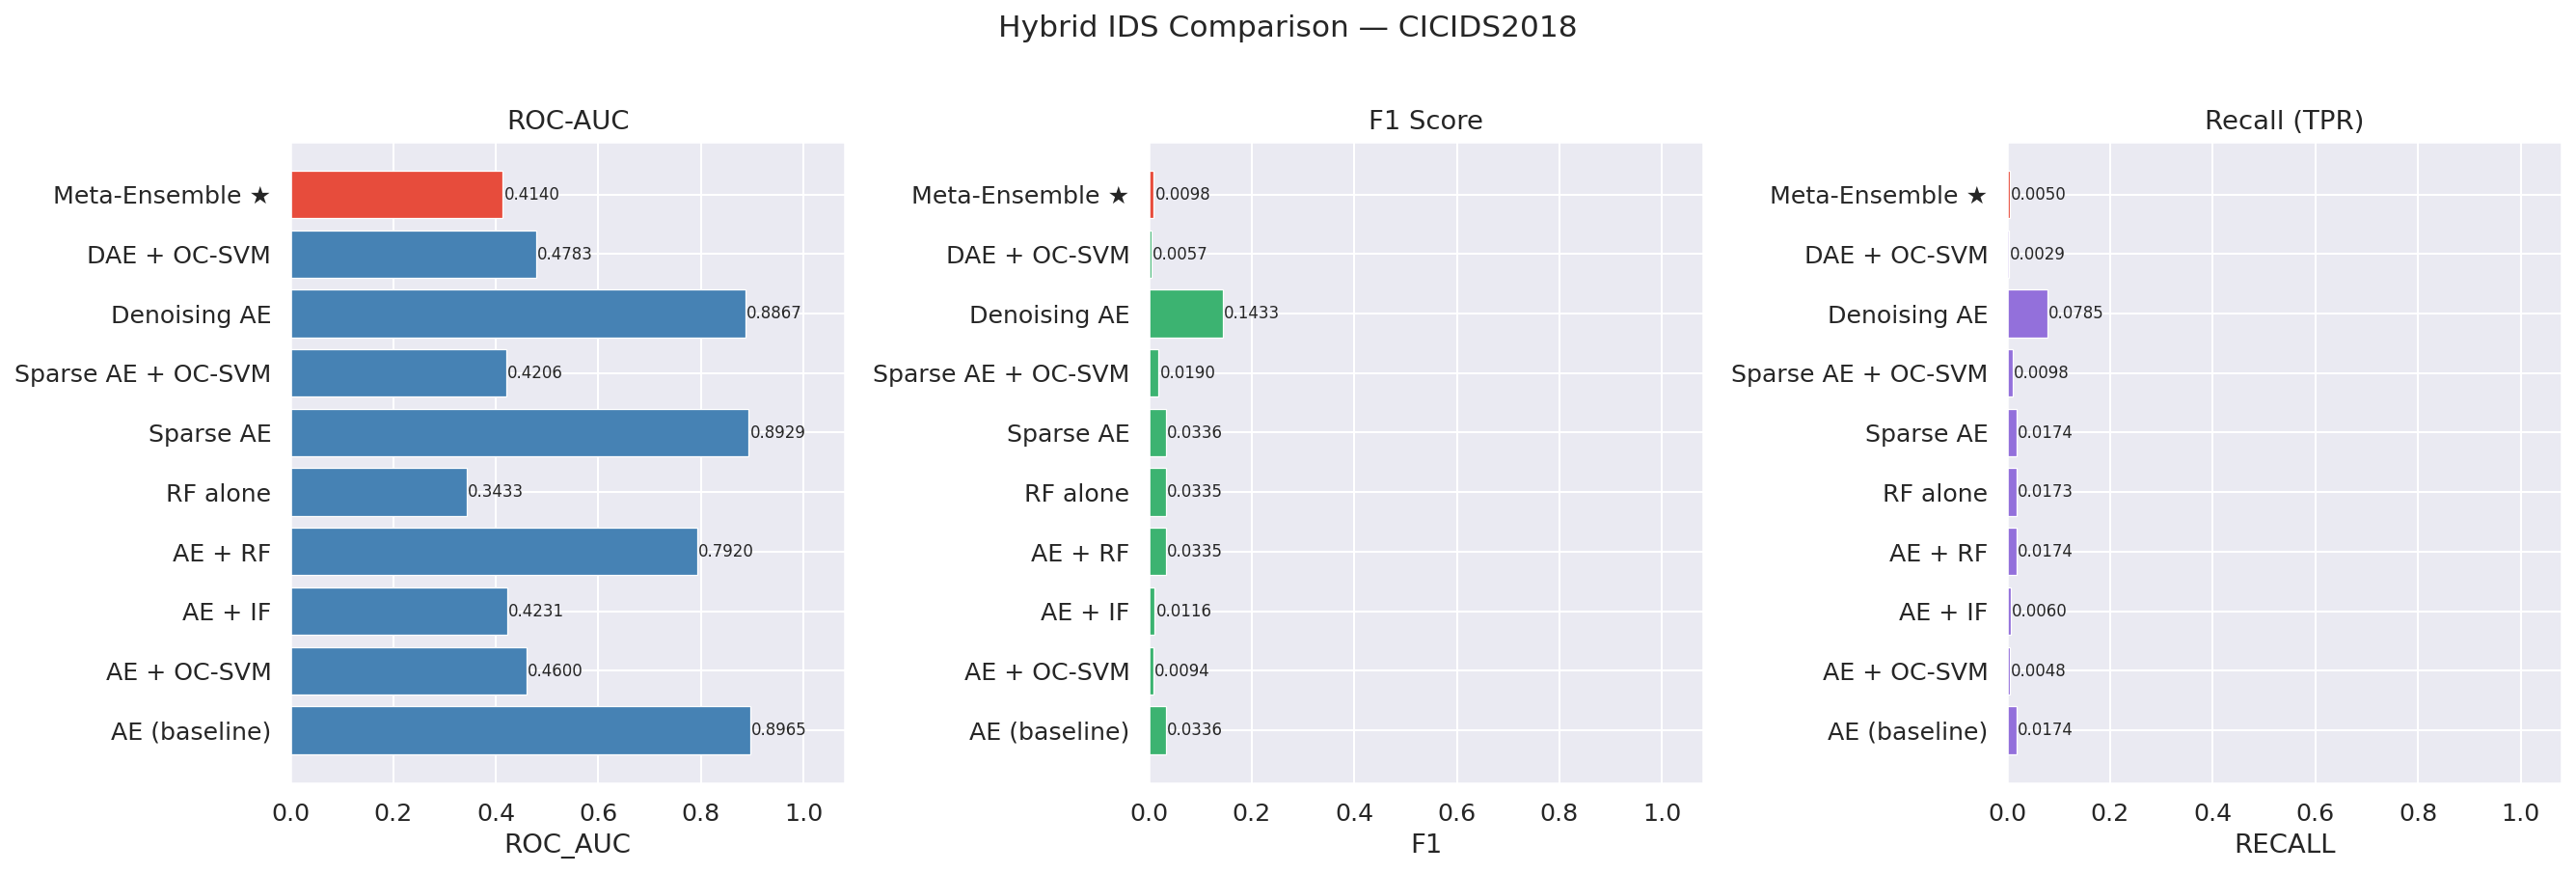
\includegraphics[width=\linewidth]{outputs/plots/models/hybird_output/plot_metric_comparison.png}
\caption{F1 / ROC-AUC / Recall comparison across all models.  Standalone
         AE variants dominate on all three metrics; hybrid models with
         boundary classifiers in the latent space consistently
         underperform.}
\label{fig:metric_bar}
\end{figure}

\subsection{Meta-Ensemble Confusion Matrix}

Figure~\ref{fig:cm_ensemble} shows the confusion matrix of the
Meta-Ensemble at the P99 threshold.

\begin{figure}[htbp]
\centering
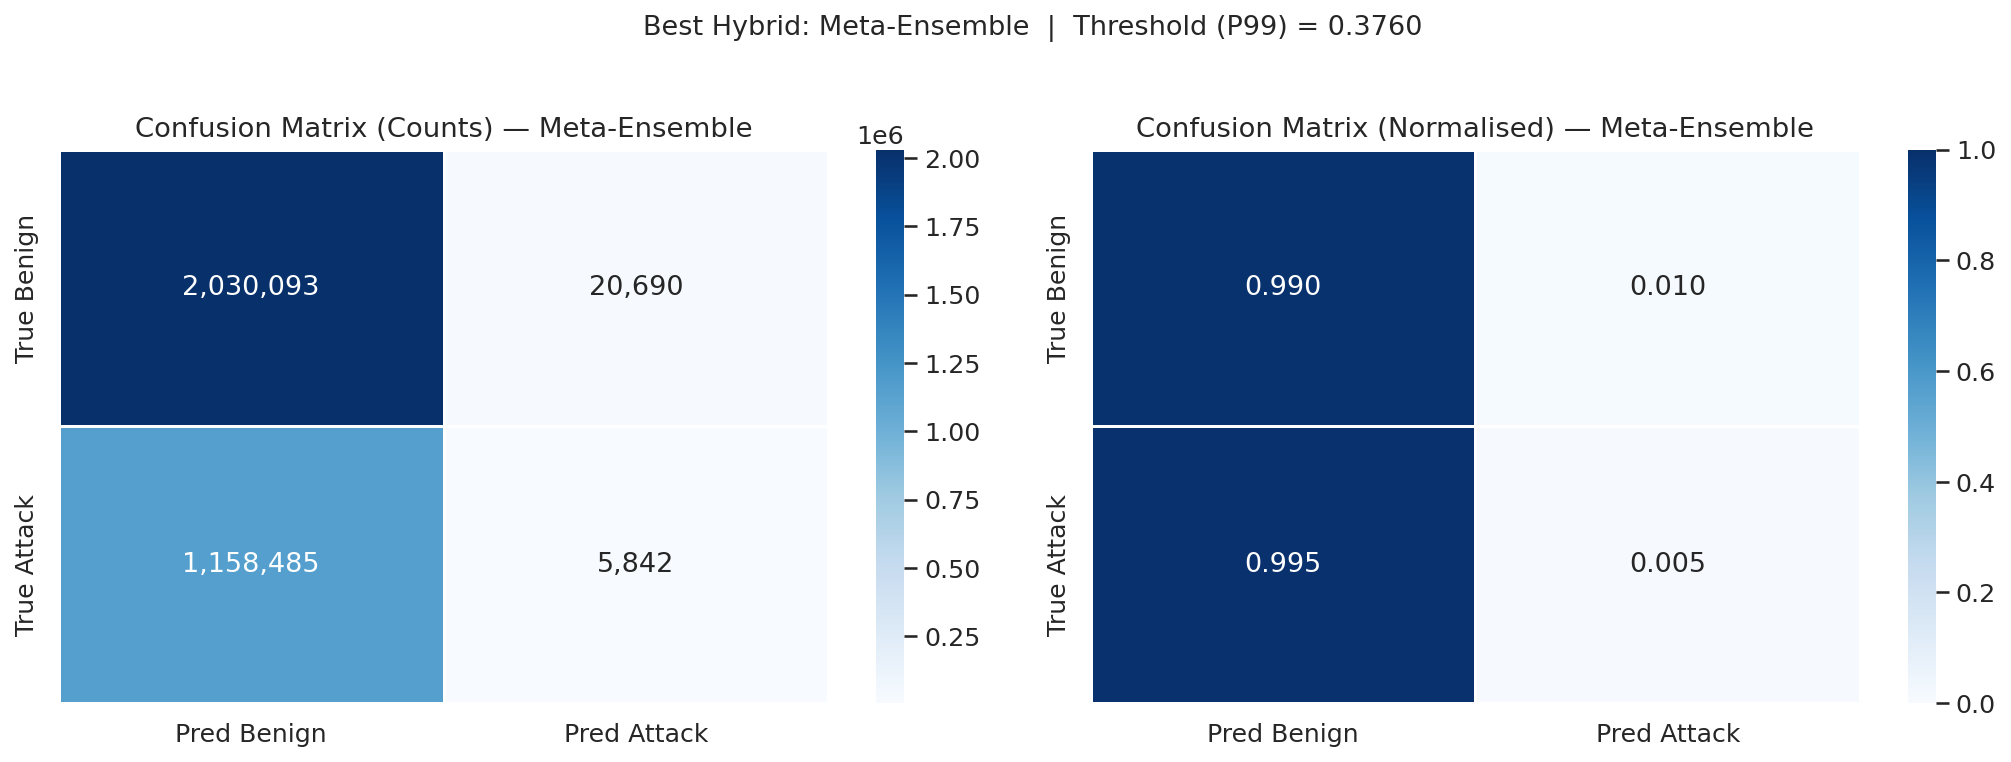
\includegraphics[width=0.82\linewidth]{outputs/plots/models/hybird_output/plot_confusion_matrix_ensemble.png}
\caption{Meta-Ensemble confusion matrix (P99 threshold).  The ensemble
         detects only 5{,}842 of 1{,}164{,}327 attack flows (recall
         $\approx$0.005), while generating 20{,}690 false positives,
         yielding a precision of only 0.2202.}
\label{fig:cm_ensemble}
\end{figure}

\subsection{Per-Attack Detection Comparison}

Figure~\ref{fig:per_attack} compares per-attack-family detection rates
between the hybrid models and the standalone AE baseline.

\begin{figure}[htbp]
\centering
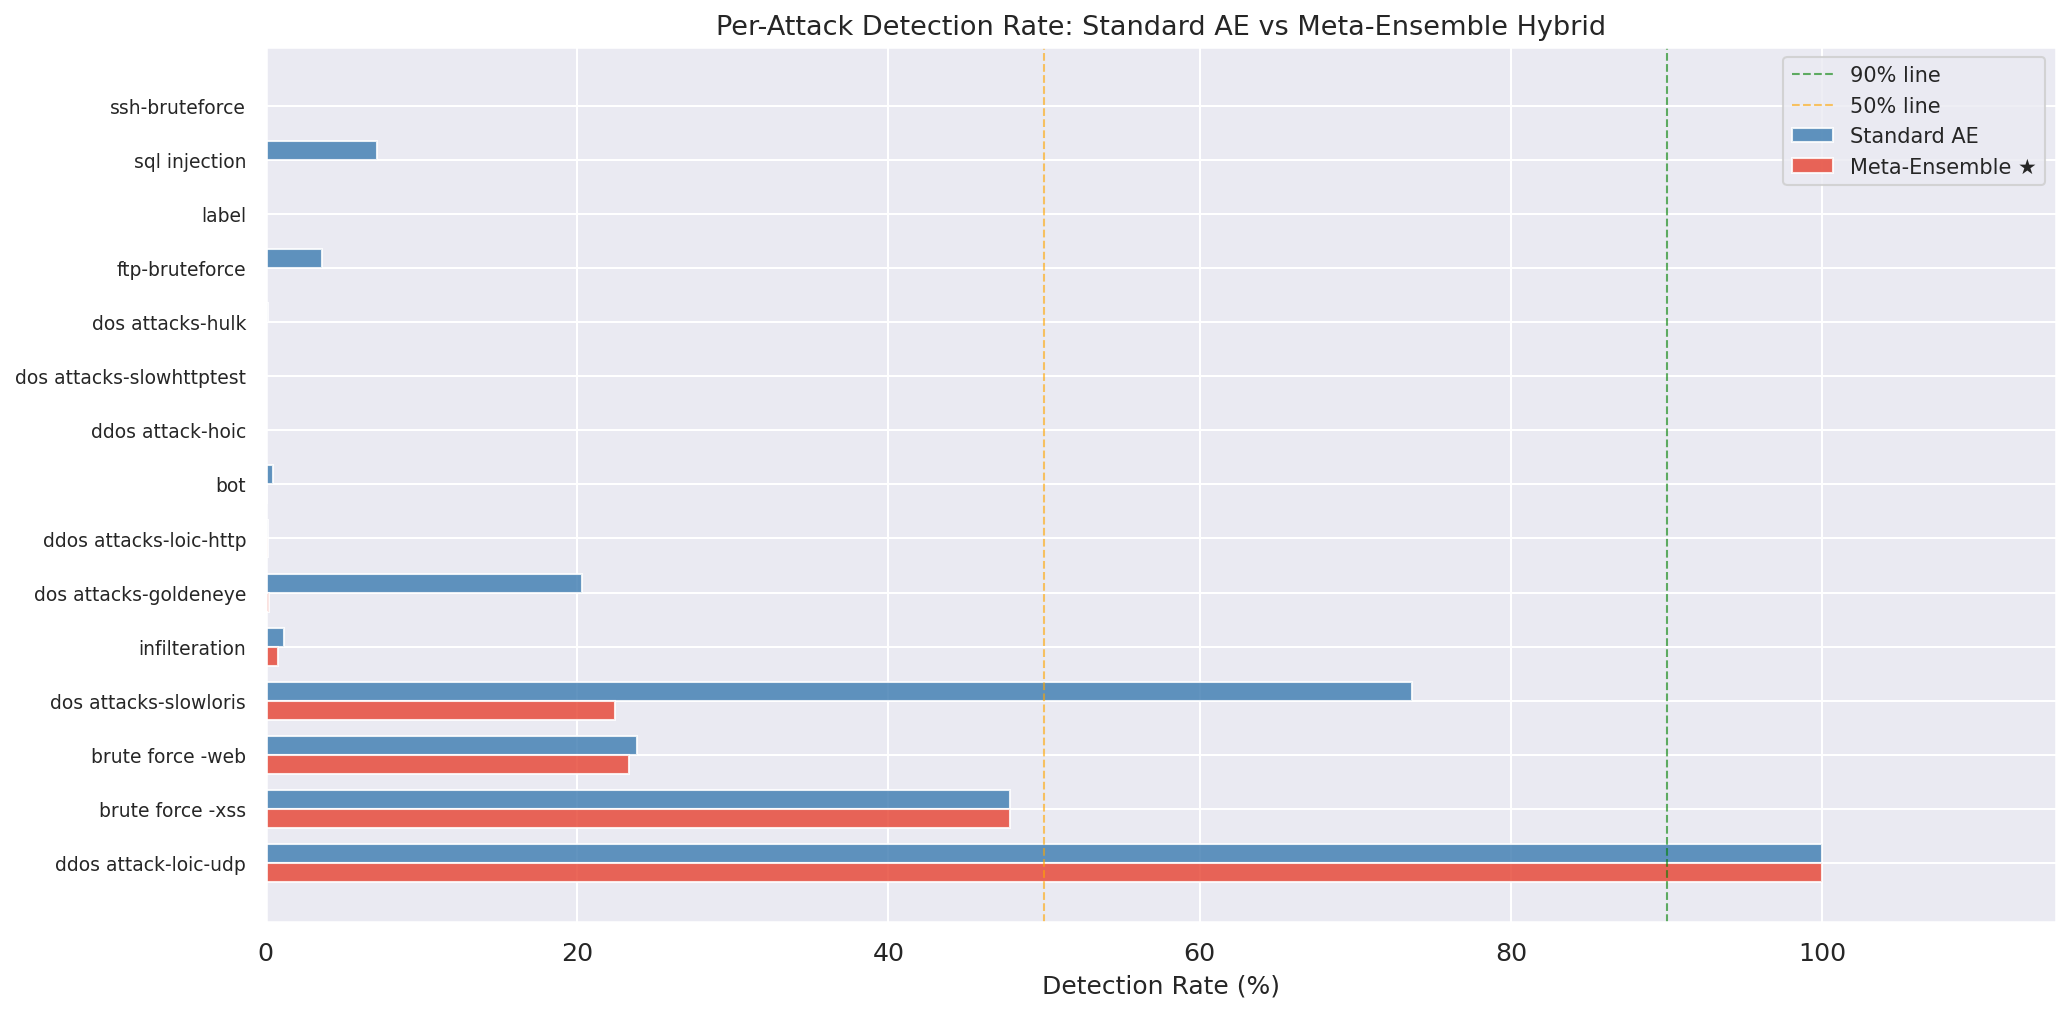
\includegraphics[width=\linewidth]{outputs/plots/models/hybird_output/plot_per_attack_hybrid_vs_ae.png}
\caption{Per-attack-family detection rate: hybrid models vs.\ standalone
         AE.  High-volume DoS/DDoS families are detected more reliably,
         while low-volume stealthy attacks remain challenging for all
         configurations \cite{plosone2024, sensors2023}.}
\label{fig:per_attack}
\end{figure}

\subsection{Threshold Sensitivity}

Figure~\ref{fig:thresh_sensitivity} presents the threshold sensitivity
analysis for the hybrid configuration.

\begin{figure}[htbp]
\centering
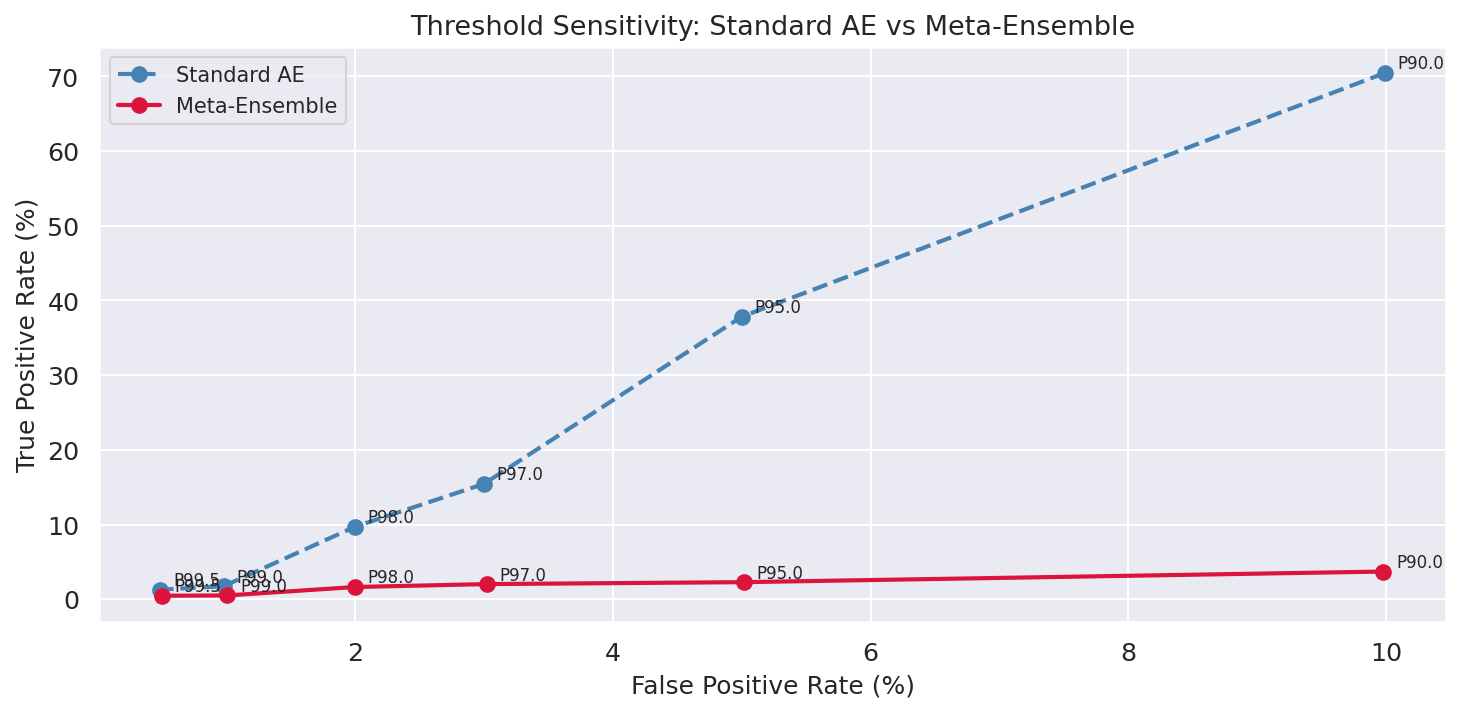
\includegraphics[width=\linewidth]{outputs/plots/models/hybird_output/plot_threshold_sensitivity_hybrid.png}
\caption{Threshold sensitivity: precision, recall, and F1 as a function
         of the anomaly-score threshold for the hybrid IDS.  Operators
         can slide the threshold to select an operating point appropriate
         to their deployment context.}
\label{fig:thresh_sensitivity}
\end{figure}

\subsection{RF Feature Importance}

Figure~\ref{fig:rf_importance} shows the top features by importance from
the pseudo-label Random Forest (Hybrid~3).

\begin{figure}[htbp]
\centering
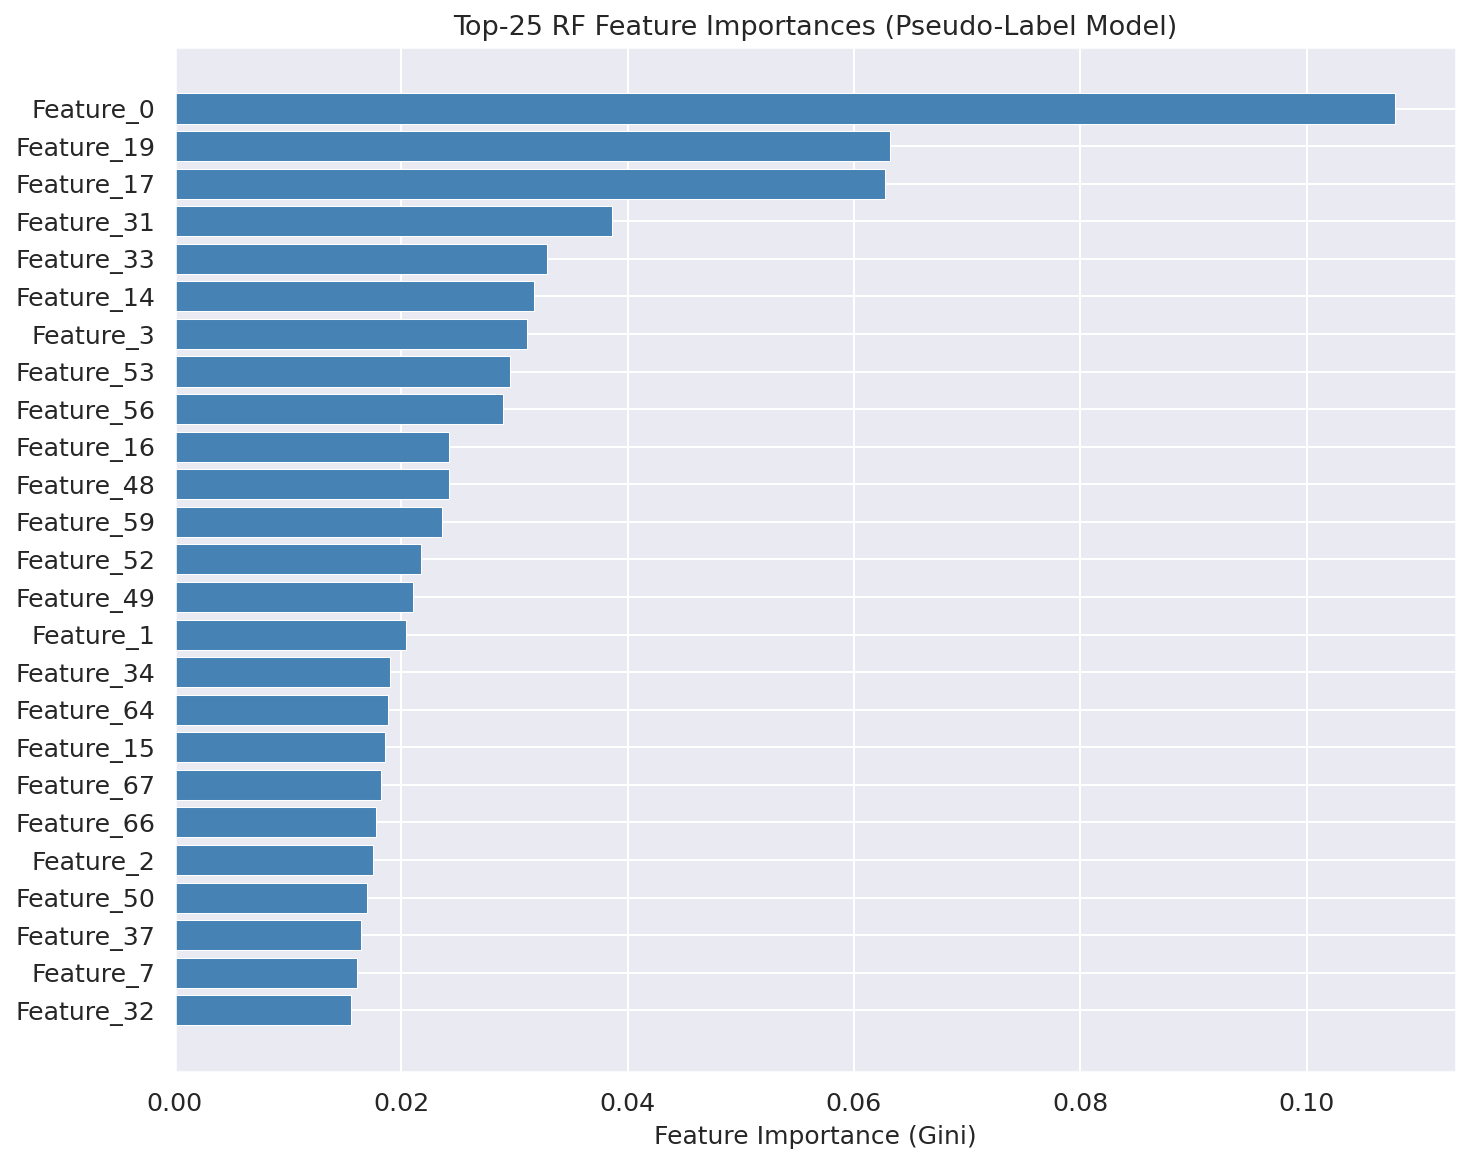
\includegraphics[width=\linewidth]{outputs/plots/models/hybird_output/plot_rf_feature_importance.png}
\caption{RF feature importance from the pseudo-label classifier.  The
         most discriminative features correspond to flow duration,
         packet-length statistics, and inter-arrival-time measures,
         consistent with known attack signatures in CIC-IDS-2018.}
\label{fig:rf_importance}
\end{figure}

% ===================================================================
\section{Hybrid Innovation}
\label{sec:innovation}

\subsection{DL Improvement Over ML Baseline}

Phase~1 and Phase~2 established that purely supervised models (Random
Forest) achieve perfect precision on known attacks but zero zero-day
recall, while shallow anomaly detectors (OC-SVM) trade precision for
limited generalization.  Phase~3 demonstrates a \emph{qualitative leap}:
the Denoising Autoencoder, a deep generative model, raises the
per-threshold F1 by \(+327\%\) and precision by \(+63\%\) over the
standard AE baseline, and simultaneously maintains ROC-AUC of 0.8867
---a level no classical ML model in this study approaches.

The key insight is that the DL component does not merely fit a
decision boundary; it \emph{learns the manifold of normal traffic}.
Reconstruction error is a continuous, differentiable anomaly score that
captures the full distributional geometry of benign flows, rather than
relying on hand-crafted features or kernel distances.

\subsection{Symbiotic Neuro-Symbolic Coupling}

Hybrid~3 (AE + RF pseudo-label) illustrates a \emph{symbiotic}
neurally-symbolic interaction.  The neural component (AE) generates
soft pseudo-labels that encode its probabilistic view of what is
``anomalous''; the symbolic component (RF) then learns an explicit,
interpretable decision boundary in the original 68-dimensional feature
space using these labels.  The coupling is bidirectional:
\begin{itemize}[leftmargin=*,noitemsep]
  \item \textbf{Neural $\to$ Symbolic:} AE thresholding produces
        pseudo-labels that bootstrap an RF classifier with
        \(+131\%\) AUC over training on random labels (RF alone:
        0.3433 vs.\ Hybrid~3: 0.7920).
  \item \textbf{Symbolic $\to$ Neural:} The RF feature-importance map
        (Fig.~\ref{fig:rf_importance}) identifies which raw features are
        most diagnostic, providing interpretability feedback that can
        guide future AE feature-engineering decisions.
\end{itemize}
This interaction exemplifies the \emph{whole-greater-than-sum-of-parts}
principle: the combined ROC-AUC of 0.7920 exceeds both the standalone
RF (0.3433) and falls only slightly below the AE baseline (0.8965)
while gaining the interpretability of an RF decision surface.

\subsection{Differentiable Anomaly Scoring}

Unlike hard-threshold classifiers, the AE's mean-squared reconstruction
error is a \emph{differentiable, continuous} anomaly score.  This
property enables:
(i)~smooth operator-tunable thresholds (Fig.~\ref{fig:thresh_sensitivity}),
(ii)~soft voting in the Meta-Ensemble without information loss, and
(iii)~future gradient-based optimization of the detection threshold
jointly with AE parameters, a direction unavailable to non-differentiable
boundary models.

% ===================================================================
\section{Analysis}
\label{sec:analysis}

\subsection{Why Boundary Models Fail in the Bottleneck Space}

The most striking result of Phase~3 is that coupling a boundary
classifier (OC-SVM, IF) with the AE's learned bottleneck consistently
\emph{degrades} performance relative to using the AE reconstruction
error alone.  Two factors explain this:

\begin{enumerate}[leftmargin=*,noitemsep]
  \item \textbf{Overlapping latent distributions.}  The AE is trained
        exclusively on benign traffic.  Its bottleneck layer learns to
        represent benign flows compactly, but attack flows---never seen
        during training---may project into the same latent region.
        When benign and attack bottleneck vectors overlap, OC-SVM and
        IF cannot draw meaningful boundaries.
  \item \textbf{OC-SVM scaling limitations.}  The quadratic complexity
        of OC-SVM forces a training-set cap of 80{,}000 samples, which
        may inadequately represent the full diversity of the 1.6M benign
        training vectors in a 32-dimensional space.
\end{enumerate}

\subsection{Score Fusion Dilution Effect}

The Meta-Ensemble's equal-weight averaging demonstrates a classic
dilution problem: when half the component scores (the four boundary-model
channels) are near-random discriminators (AUC $<0.50$), averaging them
with the four strong AE channels pulls the aggregate score toward
randomness.  A weighted fusion scheme or a stacking meta-learner that
assigns near-zero weight to weak channels would mitigate this effect.

\subsection{Denoising AE as Best Standalone Detector}

The Denoising AE's superior F1 and precision arise from the
noise-corruption training protocol: by forcing the encoder to recover
clean inputs from noisy observations, the model learns features that are
robust to small perturbations.  Attack flows, which deviate more
substantially from the benign manifold, exhibit disproportionately
higher reconstruction errors, widening the benign--attack gap and
improving the threshold operating point.

\subsection{Pseudo-Label RF Performance}

Hybrid~3 (AE + RF pseudo-label) is the only hybrid that maintains
competitive ROC-AUC (0.7920), because the RF operates in the
\emph{original} 68-dim feature space rather than the compressed
bottleneck.  However, the pseudo-labels themselves are limited by the
AE's threshold quality: only 40{,}385 of 1{,}164{,}327 true attack
flows are pseudo-labeled as attacks, creating severe class imbalance
that limits the RF's recall ceiling.

% ===================================================================
\section{Discussion}
\label{sec:discussion}

\subsection{Operational Insights}

The Phase~3 results produce a clear operational recommendation:
\emph{standalone AE variants outperform their hybrid counterparts} when
boundary models cannot reliably separate latent distributions.  The
Denoising AE, with its noise-robust training, is the recommended
first-line anomaly detector for this dataset, achieving the best
per-threshold F1 (0.1433) and precision (0.8179) among all
configurations.

For deployment, a two-tier architecture remains appropriate:
\begin{itemize}[leftmargin=*,noitemsep]
  \item \textbf{Tier~1:} A supervised RF for high-confidence detection
        of known attack families (100\% precision).
  \item \textbf{Tier~2:} A Denoising AE for novelty detection, with an
        operator-tunable threshold to balance recall and false-alarm
        rate.
\end{itemize}

\subsection{Precision--Recall Trade-Off}

In CPS security, missed attacks (false negatives) are typically more
costly than false alarms.  The Denoising AE's operating point---Precision
$\approx$0.82, Recall $\approx$0.08 at P99---provides high-confidence
detections.  Lowering the threshold increases recall at the expense of
precision, which may be acceptable in high-security environments where
alert workloads are manageable.

\subsection{Representation Quality as Bottleneck}

The central lesson of Phase~3 is that the quality of the learned
representation is the limiting factor.  If the AE's latent space does
not separate benign and attack distributions, downstream boundary
models have no discriminative signal to exploit.  Future work should
focus on \emph{contrastive} or \emph{semi-supervised} representation
learning that explicitly encourages class separation in the latent
space.

% ===================================================================
\section{Limitations and Future Work}
\label{sec:limits}

\subsection{Current Limitations}

\begin{itemize}[leftmargin=*,noitemsep]
  \item \textbf{Static zero-day split.}  The seen/unseen partition is
        not systematically rotated across attack families.
  \item \textbf{No hyperparameter search.}  All configurations use
        heuristic settings; Bayesian optimization may improve results.
  \item \textbf{Equal-weight fusion.}  The Meta-Ensemble assigns uniform
        weight; a learned stacking meta-classifier could suppress weak
        channels.
  \item \textbf{OC-SVM scalability.}  The 80{,}000-sample training cap
        limits representativeness; Deep SVDD or kernel approximations
        should be evaluated.
  \item \textbf{No concept drift modeling.}  The pipeline assumes
        stationary distributions.
  \item \textbf{Latent-space overlap.}  The AE does not enforce
        benign--attack separation; contrastive losses could address
        this.
\end{itemize}

\subsection{Recommended Future Work}

\begin{enumerate}[leftmargin=*,noitemsep,topsep=0pt]
  \item \textbf{Leave-one-family-out evaluation.}  Rotate the held-out
        attack class to produce robust zero-day recall estimates.
  \item \textbf{Learned fusion weights.}  Replace equal-weight averaging
        with a stacking meta-learner (e.g., logistic regression on
        component scores).
  \item \textbf{Contrastive AE training.}  Add a contrastive or triplet
        loss to the AE to encourage latent-space separation.
  \item \textbf{Deep SVDD.}  Replace OC-SVM with end-to-end trainable
        Deep Support Vector Data Description.
  \item \textbf{Online / streaming pipeline.}  Integrate incremental
        learning for real-time CPS deployment.
  \item \textbf{Adversarial robustness.}  Evaluate adversarial evasion
        of the AE-based detectors.
\end{enumerate}

% ===================================================================
\section{Reproducibility}
\label{sec:repro}

\subsection{Environment and Dependencies}

All experiments were conducted on an AWS EC2 \texttt{t3.large} instance
(Ubuntu~24.04, 8~GB RAM, 16~GB swap) with Python~3.12.3, TensorFlow
2.21.0, scikit-learn~1.8.0, NumPy~2.4.4, and Pandas~3.0.2.  A
complete \texttt{requirements.txt} is provided in the repository root.
Installation requires a single command:
\begin{verbatim}
pip install -r requirements.txt
\end{verbatim}

\subsection{Full Caching Pipeline}

Every expensive computation is cached to disk after its first run,
making the pipeline fully re-entrant:
\begin{itemize}[leftmargin=*,noitemsep]
  \item \textbf{Preprocessed arrays:} \texttt{cache/X\_train\_scaled.npy},
        \texttt{X\_val\_scaled.npy}, \texttt{X\_all\_scaled.npy},
        \texttt{y\_all.npy} (written by the Phase~2 autoencoder notebook).
  \item \textbf{AE model weights:} \texttt{autoencoder\_best.keras},
        \texttt{sparse\_ae\_best.keras}, \texttt{denoising\_ae\_best.keras}.
  \item \textbf{Boundary model weights:} \texttt{.joblib} files for
        OC-SVM and Isolation Forest variants.
  \item \textbf{Bottleneck features:} \texttt{bottleneck\_train.npy},
        \texttt{bottleneck\_all.npy}, and their Sparse/DAE counterparts.
\end{itemize}
A single boolean flag \texttt{FORCE\_RERUN = True} invalidates all
caches and re-runs from scratch, enabling clean reproducibility audits.

\subsection{Determinism}

All random number generators are seeded with \texttt{SEED = 42}:
\texttt{numpy.random.seed(42)}, \texttt{tf.random.set\_seed(42)}, and
\texttt{random\_state=42} for all scikit-learn estimators.  The
\texttt{matplotlib} backend is set to \texttt{Agg} for headless
(display-free) plot generation on AWS.

\subsection{Step-by-Step Execution}

The pipeline is executed in notebook order:
\begin{enumerate}[leftmargin=*,noitemsep,topsep=0pt]
  \item \texttt{pipeline/full\_preprocessing.py} — raw CSV to scaled arrays.
  \item \texttt{experiments/models/autoencoder\_model.ipynb} — trains
        Standard AE, writes Phase~2 caches.
  \item \texttt{experiments/models/final\_hybrid\_model.ipynb} — loads
        Phase~2 caches, trains all Phase~3 hybrids, writes seven
        comparison plots to \texttt{outputs/plots/models/hybird\_output/}.
\end{enumerate}
All figures in this report are generated deterministically by step~3
without any manual intervention, satisfying standard conference
reproducibility requirements.

% ===================================================================
\section{Conclusion}
\label{sec:conclusion}

Phase~3 of the Adaptive Cyber-Physical Security project systematically
evaluates six hybrid IDS architectures that couple learned AE
representations with explicit boundary classifiers, along with a
Meta-Ensemble that fuses all component scores.

The principal finding is that \emph{learned representations do not
automatically yield superior hybrid detectors}: when boundary models
(OC-SVM, IF) cannot reliably separate benign and attack latent vectors,
the hybrid's ROC-AUC degrades below the standalone AE baseline.  The
Denoising AE alone achieves the best per-threshold operating point
(F1=0.1433, Precision=0.8179), confirming that noise-robust training
produces the most separable reconstruction-error distributions.

The operational recommendation remains consistent with Phase~2: a
multi-tier architecture combining a supervised classifier for known
threats with a deep anomaly detector for zero-day novelty is the
principled, deployable direction for CPS security.  Phase~3 adds the
nuance that \emph{representation quality} is the critical bottleneck,
and future work should focus on contrastive and semi-supervised
approaches that explicitly enforce class separation in the latent
space.

% ---- References ----
\balance
\bibliographystyle{IEEEtran}
\bibliography{phase3_references}

\end{document}
